% Edit distance table (generated by figs_c2ch05.py).
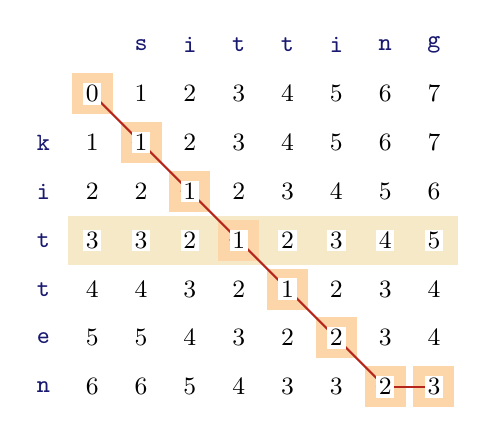
\begin{tikzpicture}[x=0.62cm,y=0.62cm,every node/.style={font=\small}]
\fill[Goldenrod!25] (-0.5,-3.5) rectangle (7.5,-2.5);
\fill[BurntOrange!30] (6.58,-6.42) rectangle (7.42,-5.58);
\fill[BurntOrange!30] (5.58,-6.42) rectangle (6.42,-5.58);
\fill[BurntOrange!30] (4.58,-5.42) rectangle (5.42,-4.58);
\fill[BurntOrange!30] (3.58,-4.42) rectangle (4.42,-3.58);
\fill[BurntOrange!30] (2.58,-3.42) rectangle (3.42,-2.58);
\fill[BurntOrange!30] (1.58,-2.42) rectangle (2.42,-1.58);
\fill[BurntOrange!30] (0.58,-1.42) rectangle (1.42,-0.58);
\fill[BurntOrange!30] (-0.42,-0.42) rectangle (0.42,0.42);
\draw[BrickRed,thick,<-] (7,-6) -- (6,-6);
\draw[BrickRed,thick,<-] (6,-6) -- (5,-5);
\draw[BrickRed,thick,<-] (5,-5) -- (4,-4);
\draw[BrickRed,thick,<-] (4,-4) -- (3,-3);
\draw[BrickRed,thick,<-] (3,-3) -- (2,-2);
\draw[BrickRed,thick,<-] (2,-2) -- (1,-1);
\draw[BrickRed,thick,<-] (1,-1) -- (0,0);
\node[fill=white,inner sep=1pt] at (0,0) {0};
\node[fill=white,inner sep=1pt] at (1,0) {1};
\node[fill=white,inner sep=1pt] at (2,0) {2};
\node[fill=white,inner sep=1pt] at (3,0) {3};
\node[fill=white,inner sep=1pt] at (4,0) {4};
\node[fill=white,inner sep=1pt] at (5,0) {5};
\node[fill=white,inner sep=1pt] at (6,0) {6};
\node[fill=white,inner sep=1pt] at (7,0) {7};
\node[fill=white,inner sep=1pt] at (0,-1) {1};
\node[fill=white,inner sep=1pt] at (1,-1) {1};
\node[fill=white,inner sep=1pt] at (2,-1) {2};
\node[fill=white,inner sep=1pt] at (3,-1) {3};
\node[fill=white,inner sep=1pt] at (4,-1) {4};
\node[fill=white,inner sep=1pt] at (5,-1) {5};
\node[fill=white,inner sep=1pt] at (6,-1) {6};
\node[fill=white,inner sep=1pt] at (7,-1) {7};
\node[fill=white,inner sep=1pt] at (0,-2) {2};
\node[fill=white,inner sep=1pt] at (1,-2) {2};
\node[fill=white,inner sep=1pt] at (2,-2) {1};
\node[fill=white,inner sep=1pt] at (3,-2) {2};
\node[fill=white,inner sep=1pt] at (4,-2) {3};
\node[fill=white,inner sep=1pt] at (5,-2) {4};
\node[fill=white,inner sep=1pt] at (6,-2) {5};
\node[fill=white,inner sep=1pt] at (7,-2) {6};
\node[fill=white,inner sep=1pt] at (0,-3) {3};
\node[fill=white,inner sep=1pt] at (1,-3) {3};
\node[fill=white,inner sep=1pt] at (2,-3) {2};
\node[fill=white,inner sep=1pt] at (3,-3) {1};
\node[fill=white,inner sep=1pt] at (4,-3) {2};
\node[fill=white,inner sep=1pt] at (5,-3) {3};
\node[fill=white,inner sep=1pt] at (6,-3) {4};
\node[fill=white,inner sep=1pt] at (7,-3) {5};
\node[fill=white,inner sep=1pt] at (0,-4) {4};
\node[fill=white,inner sep=1pt] at (1,-4) {4};
\node[fill=white,inner sep=1pt] at (2,-4) {3};
\node[fill=white,inner sep=1pt] at (3,-4) {2};
\node[fill=white,inner sep=1pt] at (4,-4) {1};
\node[fill=white,inner sep=1pt] at (5,-4) {2};
\node[fill=white,inner sep=1pt] at (6,-4) {3};
\node[fill=white,inner sep=1pt] at (7,-4) {4};
\node[fill=white,inner sep=1pt] at (0,-5) {5};
\node[fill=white,inner sep=1pt] at (1,-5) {5};
\node[fill=white,inner sep=1pt] at (2,-5) {4};
\node[fill=white,inner sep=1pt] at (3,-5) {3};
\node[fill=white,inner sep=1pt] at (4,-5) {2};
\node[fill=white,inner sep=1pt] at (5,-5) {2};
\node[fill=white,inner sep=1pt] at (6,-5) {3};
\node[fill=white,inner sep=1pt] at (7,-5) {4};
\node[fill=white,inner sep=1pt] at (0,-6) {6};
\node[fill=white,inner sep=1pt] at (1,-6) {6};
\node[fill=white,inner sep=1pt] at (2,-6) {5};
\node[fill=white,inner sep=1pt] at (3,-6) {4};
\node[fill=white,inner sep=1pt] at (4,-6) {3};
\node[fill=white,inner sep=1pt] at (5,-6) {3};
\node[fill=white,inner sep=1pt] at (6,-6) {2};
\node[fill=white,inner sep=1pt] at (7,-6) {3};
\node[MidnightBlue] at (1,1) {\texttt{s}};
\node[MidnightBlue] at (2,1) {\texttt{i}};
\node[MidnightBlue] at (3,1) {\texttt{t}};
\node[MidnightBlue] at (4,1) {\texttt{t}};
\node[MidnightBlue] at (5,1) {\texttt{i}};
\node[MidnightBlue] at (6,1) {\texttt{n}};
\node[MidnightBlue] at (7,1) {\texttt{g}};
\node[MidnightBlue] at (-1,-1) {\texttt{k}};
\node[MidnightBlue] at (-1,-2) {\texttt{i}};
\node[MidnightBlue] at (-1,-3) {\texttt{t}};
\node[MidnightBlue] at (-1,-4) {\texttt{t}};
\node[MidnightBlue] at (-1,-5) {\texttt{e}};
\node[MidnightBlue] at (-1,-6) {\texttt{n}};
\end{tikzpicture}
